\chapter{Modellierung des Wasserstoff-Energiesystems}
\label{cha:Methode}
Das folgende Kapitel dokumentiert die Entwicklung des zur Simulation des Wasserstoff-Energiesystems verwendeten Modells.
Dazu wird Anfangs die Modellierung des Elektrolyseurs und der Brennstoffzelle vorgestellt. Weiterhin werden Bewertungskriterien für Konzepte des Wasserstoff-Energiesystems ausgearbeitet und anschließend alternative Systemkonzepte präsentiert. 
Im letzten Abschnitt werden die für die Simulation der Konzepte gewählte Parameter und Randbedingungen hergeleitet.

\section{Implementierung der Wasserstoffkomponenten in Modelica} 
Ziel dieser Arbeit ist ein Modell, welches in der Lage ist das Verhalten des gesamten Elektrolyse-Systems vorherzusagen. Dazu werden zusätzlich zur Elektrolyse-Zelle die relevanten Systemkomponenten in der Modellierung berücksichtigt. Als Eingangsgrößen werden dabei neben Kennwerten aus Datenblättern Literaturangaben verwendet, um die Modellierung verschiedener Anlagen der vorgestellten Technologien zu erleichtern. Der Fokus liegt dabei auf der Modellierung von alkalischen- und PEM-Zellen, da sie, wie in \ref{subsec:Technologien der Wasserelektrolyse} sowie \ref{subsec:BZ}, erläutert der aktuelle Standard sind. Der Detaillierungsgrad ist so gewählt, dass die Genauigkeit der Ergebnisse einerseits eine stichhaltige Bewertung der Konzepte des Wasserstoff-Energiesystems ermöglicht und andererseits die Rechendauer in einem akzeptablen Bereich liegt.
Weiterhin ist eine Betrachtung des Wärmehaushalts für die Brennstoffzelle zur Modellierung der Kraft-Wärme-Kopplung implementiert.\\

Modelica ist eine objektorientierte Modellierungssprache, mit deren Hilfe Systeme durch gewöhnliche Differentialgleichungen in Kombination  mit diskreten Vorfällen beschrieben werden. Nach \citet{schamai_modelica_2009} ist Modelica daher ideal für die Modellierung von physikalischen Systemen mit Energieaustausch und weiteren zeitkontinuierlichen Vorgängen geeignet. Das Modell wurde in Modelica 4.0.0 in der Entwicklungsumgebung Dymola 2021x entwickelt.\\


\subsection{Modellierung der Zelle}\ \\
\label{subsec:Modellierung der Zelle}

Als Modellarchitektur wird ein Aufbau mit einem partiellen Modell gewählt (Abbildung \ref{fig:Modellstruktur}), da die Beschreibung der idealen Zellspannung und die Approximationen der Verlustmechanismen für Elektrolyseur und Brennstoffzelle identisch sind. \begin{figure}[h]
	\centering
		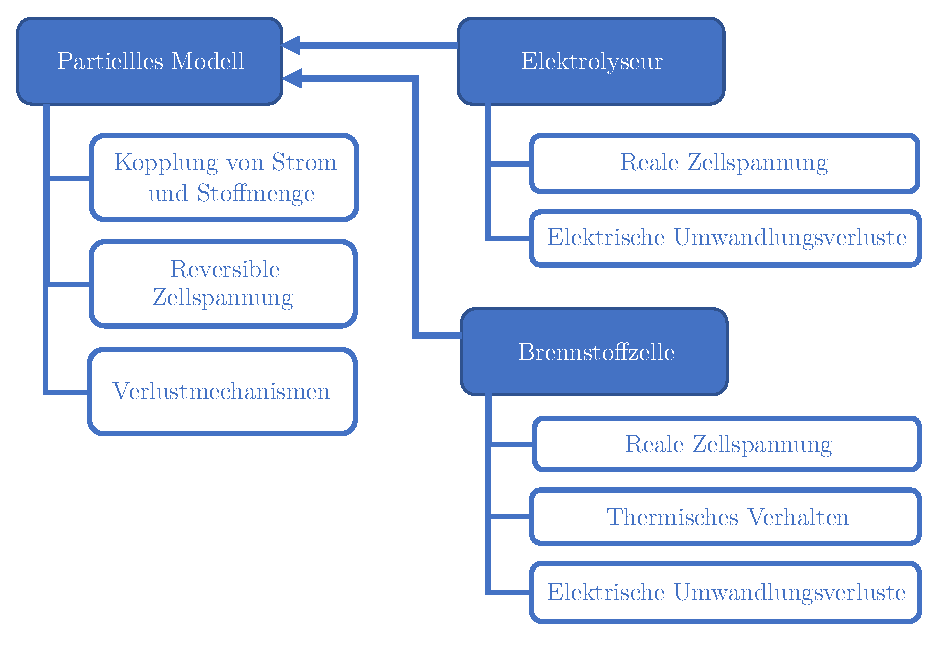
\includegraphics[scale=1]{Figures/Modellstruktur}
		\caption{Struktur des entwickelten Modells.}
\label{fig:Modellstruktur}	
\end{figure}
Im partiellen Modell sind daher daher folgende Zusammenhänge implementiert: Erstens der Zusammenhang von Strom und produzierter Stoffmenge (Gleichung \ref{gl:n_i}), zweitens die Gleichungen zur Berechnung der idealen Zellspannung (Gleichung \ref{gl:Urev} sowie der Temperatur- und Druckeinfluss) und drittens die Berechnung der Aktivierungsverluste  (Gleichung  \ref{gl:Akt}) und Ohmschen Überspannungen (für PEM-Zellen Gleichung \ref{gl:Ohm2}, sonst \ref{gl:Ohm}). Die Technologie der Zelle wird im Modell über den  ausgewählt, der die Zustände "\textit{alk}" (für die alkalische Bauart), "\textit{pem}" (Bei Verwendung einer Protonen Austausch Membran) oder "\textit{so}" (für Festoxid-Zellen) annehmen kann.
Für die Bauarten sind im Modell verschiedene Werte für die Parametern $i_0, \alpha, \delta$ und $\sigma$ hinterlegt. Abhängig vom "\textit{Bauart}"-Parameter werden diese zur Berechnung der Verluste genutzt.\\

Die Modelle für Elektrolyseur und Brennstoffzelle enthalten die Gleichungen zur Berechnung der realen Zellspannung (Gleichung \ref{gl:U_realEL} beziehungsweise \ref{gl:U_real-BZ}) sowie die Approximationen der in \ref{subsec:Systemkomponenten} erläuterten Umwandlungsverluste. Diese werden im Modell als über den Betriebsbereich konstant angenommen. Das erweist sich unter Beachtung des von \citet[S.~50]{tjarks_pem-elektrolyse-systeme_2017} angeführten Verlaufs des Wirkungsgrades eines Gleichrichters insbesondere im oberen Lastbereich als akzeptable Näherung. Auch auf den von \citet{trubitsyn_high-efficiency_2010} untersuchten Wechselrichter trifft diese Aussage zu.\\

Das Brennstoffzellenmodell enthält darüber hinaus die Berechnung der zur Verfügung stehenden Abwärme:\\
Die Anfahrzeit von Elektrolysezellen liegt aus dem Stand-by nach \citet{milanzi_technischer_2018} bei $10-\SI{30}{\s}$, was im Vergleich zu den für die Simulation verwendeten Zeitschritten ($\SI{900}{\s}$) als vernachlässigbar angenommen wird. Daher werden im Rahmen dieser Arbeit dynamische Vorgänge, die insbesondere durch die  Betriebstemperatur der Zelle beeinflusst werden \citep{garcia-valverde_simple_2012}, nicht betrachtet.\\
Zur Modellierung des thermischen Verhaltens wird somit vereinfachend angenommen, dass die Betriebstemperatur stets konstant ist. Daher wird die Energiebilanz \ref{gl:Energiebilanz} wie folgt vereinfacht:

\begin{align}
0 = (\dot{n}_{H2} \cdot c_{p, H2} + \dot{n}_{Luft} \cdot c_{p, Luft}) \cdot (T_{Umgebung} - T) + I \cdot (U_{tn} - U_{Zell}) - \dot{Q}
\end{align}

Der Wärmestrom $\dot{Q}$ setzt sich aus den Wärmeverlusten $\dot{Q}_{Verlust}$ und der nutzbaren Abwärme $\dot{Q}_{Nutz}$ zusammen. Die Wärmeverluste werden über den Wärmeverlustfaktor $C_{th}$ bestimmt:

\begin{align}
\dot{Q}_{Verlust} = C_{th} \cdot (T - T_{Umgebung}) 
\end{align}

\section{Entwicklung von Energiesystem-Konzepten}
Im folgenden Abschnitt werden anfangs die zur Bewertung der Systemkonzepte genutzten Parameter erläutert. Zudem werden die betrachteten Konzepte sowie die gewählte Betriebsstrategie erläutert.

\subsection{Identifikation sinnvoller Bewertungskriterien}
In \citet{reich_grundlagen_2018} werden Kriterien zum Vergleich von Energiesystemen angeführt, die eine umfassende Bewertung ermöglichen. Als für ein Unternehmen relevante Kriterien werden in dieser Arbeit Kennwerte zur ökonomische sowie ökologische Bewertung der Konzepte genutzt.\\

Zur ökonomischen Bewertung wird der Kapitalwert - eine Kennzahl der Dynamischen Investitionsrechnung \citep{muller_vorlesung_2020} - als Kriterium verwendet . 
Fällt der Kapitalwert einer Investition positiv aus, so wird diese als wirtschaftlich sinnvoll bewertet. Der Kapitalwert $C$ für einen Zeitraum von $n$ Jahren errechnet sich aus den Anfangsinvestitionen $I_0$, den jährlichen Einsparungen $Z_{ein}$ und Ausgaben $Z_{aus}$ und dem kalkulatorischen Zinssatz $i$ \citep{muller_vorlesung_2020} (Die jährlichen Einsparungen errechnen sich in dieser Arbeit aus den verminderten Strom- und Gaskosten und der Einspeisevergütung und als Ausgaben werden zusätzliche Wartungskosten gewertet):

\begin{align}
C = -I_0 + \frac{(1+i)^n-1}{(1+i)^n \cdot i} \cdot (Z_{ein} - Z_{aus})
\end{align}

Als ökologisches Bewertungskriterium dient in dieser Arbeit der eingesparte $\ce{CO2}$ Ausstoß ($\Delta m_{\ce{CO2}}$). Dieser setzt sich einerseits aus den Stromeinsparung $\Delta P_{el}$ in Verbindung mit dem $\ce{CO2}$ Faktor für den Strommix ($m_{Strom}$) und andererseits aus den Gaseinsparungen ($\Delta Q$) und dem $\ce{CO2}$ Faktor des Erdgases ($m_{Gas}$) zusammen (Als Stromeinsparungen wird in dieser Arbeit neben dem eingesparten Netzverbrauch auch die Einspeisung gewertet).  

\begin{align}
\Delta m_{\ce{CO2}} = \Delta P_{el} \cdot m_{Strom} + \Delta Q \cdot m_{Gas}
\end{align}

\subsection{Entwicklung von Systemkonzepten}
\begin{figure}[h]
	\centering
		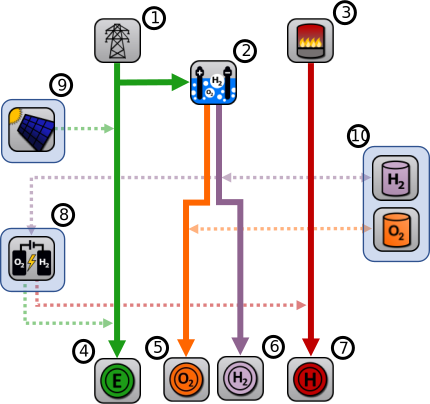
\includegraphics[scale=1]{Figures/Systemkonzepte}
		\caption{Aktuelles System sowie betrachtete Erweiterungen (1.Netzanschluss 2.Elektrolyseur 3.Gasheizung 4.Strombedarf 5.Wasserstoffbedarf 6.Sauerstoffbedarf 7.Heizwärmebedarf - Erweiterungen: 8.Brennstoffzelle 9.PV-Anlage 10.Gasspeicher).}
\label{fig:Modellstruktur}	
\end{figure}

Abbildung \ref{fig:Modellstruktur} liefert einen Überblick, über das aktuelle Wasserstoff-Energiesystem, sowie die in dieser Arbeit berücksichtigten Erweiterungen. Folgende Anforderungen werden dabei an die Systemkonzepte gestellt:\\
Der Strombedarf(4) und Heizwärmebedarf(6) muss gedeckt werden und die zum Betrieb der Veredelungsanlagen benötigte Menge an Sauerstoff(5) und Wasserstoff(6) muss bereitgestellt werden. Im Jahr $2018$ lag das Stoffmengenverhältnis des benötigten Wasserstoffs zum benötigten Sauerstoff bei $1,22:1$, für $2019$ ergab sich ein Verhältnis von $1,40:1$ (\ref{Apx:Systemkonzepte}).\\ 
Im aktuellen System wird der Strom aus dem Netz(1) bezogen und der Wärmebedarf von einer Gasheizung(3) gedeckt. Die Prozessgase werden von einem alkalischen Elektrolyseur(2) produziert und das Stoffmengenverhältnis von Wasserstoff zu Sauerstoff beträgt dabei, wie in Gleichung \ref{gl:Reaktionsgleichung} beschrieben, $2:1$.\\


Bei Konzept 1 wird das bestehende System um eine Brennstoffzelle(8) erweitert, die den Wasserstoffüberschuss zur Kraft-Wärme-Kopplung nutzt. Beim zweiten Konzept wird die Verwendung einer PV-Anlage(9) betrachtet - Konzept 3 enthält sowohl eine PV-Anlage als auch eine Brennstoffzelle. Konzept 4 beinhaltet die Erweiterung mit einer PV-Anlage in Kombination mit einem Gasspeicher(10).\\ 
    
Konzepte 1-3 werden Bedarfs-gesteuert betrieben, was auch der Betriebsstrategie im aktuellen System entspricht. Bei Konzept 4 wird im Falle von Solarstrom-Überschuss eine Einspeicherung in Form von Prozessgasen vorgenommen. Sobald der Solarstrom nicht ausreicht, um die Produktionsstätte samt Elektrolyseur zu versorgen, werden, falls vorhanden, die im Speicher gelagerten Gase den Anlagen zugeführt.

\section{Parametrierung der Komponenten}
Im folgenden Abschnitt werden die gewählten Parameter zur Simulation der Systemkonzepte vorgestellt. Dies beinhaltet einerseits die Parametrierung der Wasserstoffkomponenten und weiterhin die Verläufe des Strom, Heizwärme und Prozessgasbedarfs.

\paragraph{Alkalischer Elektrolyseur}\ \\
Im System des Quarzglasherstellers ist ein alkalischer Elektrolyseur vom Hersteller ErreDue S.p.A. mit der Modellbezeichnung G-32 verbaut. Als voreingestellte Betriebstemperatur ist $\SI{60}{\degreeCelsius}$ angegeben und der Betriebsdruck liegt standardmäßig bei $\SI{4}{\bar}$.
Für die gesamte Zellfläche liegen keine Angaben vor, daher wird diese anhand der maximal produzierten Stoffmenge und den Literaturangaben zur maximalen Stromdichte von alkalischen Elektrolyseuren abgeschätzt (siehe \ref{Apx:Modelle}). Als Elektrolyt dient 20-prozentige Natronlauge, was einer Stoffmengenkonzentration von $\SI{6,095}{\mol\per\l}$ entspricht \citep{periodensystem-online_dichtewerttabelle_nodate-1}.\\
Für den Elektrodenabstand ($\delta_{alk}$) und die Parameter $\alpha$ und $i_0$ werden die von \citet{milewski_modeling_2014} angegebenen Werte übernommen (siehe \ref{Apx:Modelle}).\\ 
Der Wirkungsgrad des von \citet[S.~50]{tjarks_pem-elektrolyse-systeme_2017} verwendeten Gleichrichters liegt bei einer Leistung von $20-\SI{100}{\%}$ in einem Bereich von $94-\SI{96}{\%}$, daher wird in dieser Arbeit ein Wirkungsgrad von $\SI{95}{\%}$ angenommen.

\begin{table}[ht]
		\centering
		\caption{Zur Simulation des alkalischen Elektrolyseurs verwendete Parameter.}
		\begin{tabular}{l c c}
		\toprule
		Betriebstemperatur & $T$ & $\SI{60}{\degreeCelsius}$\\
		Betriebsdruck & $p$ & $\SI{4}{\bar}$\\
		Gesamtfläche & $A_{ges}$ & $\SI{10,2}{\m\squared }$\\
		Elektrolytkonzentration & $m$ & $\SI{6,095}{\mol \per \l}$\\
		 & $i_0$ & $ \SI{3,15}{\A\per\m\squared}$\\
		 & $\alpha$ & $\SI{0,17}{}$\\
		Elektrodenabstand & $\delta_{alk}$ & $\SI{0,66}{\cm}$\\
		Effizienz des Gleichrichters & $\eta_{GR}$ & $\SI{95}{\%}$ \\
		\bottomrule
		\end{tabular}
		\label{tb:ParameterElektrolyseur}
\end{table}	

\paragraph{PEM-Brennstoffzelle}\ \\
Für die Simulation wird eine PEM-Brennstoffzelle verwendet, da dies, wie in \ref{subsec:BZ} angeführt, die meist verwendete Bauart bei Brennstoffzellen ist. Für die Betriebstemperatur werden $\SI{80}{\degreeCelsius}$ angenommen und für den Betriebsdruck wird der Wert des Elektrolyseurs verwendet. Die Zellfläche ist so gewählt, dass die maximal produzierte Stoffmenge des Elektrolyseurs der maximal verwendeten Stoffmenge der Brennstoffzelle gleicht (siehe \ref{Apx:Modelle}). \citet{rashid_hydrogen_2015} nennen $100-\SI{200}{\micro\m}$ als übliche Membrandicke, daher ist diese im Modell mit $\SI{150}{\micro\m}$ abgeschätzt.
Die Werte der Parameter $i_0$, $\alpha$ und $C_{th}$ sind aus der Arbeit von \citet{webster_implementation_2019} entnommen, der Wärmeverlustfaktor $C_{th}$ wird anhand der Zellfläche skaliert, um den Einfluss der Baugröße auf die Konvektionsfläche zu berücksichtigen (siehe \ref{Apx:Modelle}). 
Als Wirkungsgrad des Wechselrichters wird auf Grundlage der von \citet{trubitsyn_high-efficiency_2010} vorgestellten Daten $\SI{96}{\%}$ als Näherung angenommen.

\begin{table}[ht]
		\centering
		\caption{Zur Simulation der PEM-Brennstoffzelle verwendete Parameter.}
		\begin{tabular}{l c c}
		\toprule
		Betriebstemperatur & $T$ & $\SI{80}{\degreeCelsius}$\\
		Betriebsdruck & $p$ & $\SI{4}{\bar}$\\
		Gesamtfläche & $A_{ges}$ & $\SI{2,55}{\m\squared }$\\
		Membrandicke & $\delta_{pem}$ & $\SI{150}{\micro\m}$\\
		 & $i_0$ & $ \SI{2,16e-4}{\A\per\m\squared}$\\
		 & $\alpha$ & $0,7353$\\
		Elektrischer Widerstand & $R_{ele}$ & $\SI{0,096}{\ohm\per\cm\squared}$ \citep{tjarks_pem-elektrolyse-systeme_2017}\\	
		Wärmeverlustfaktor & $C_{th}$ & $\SI{21,939}{\W\per\K}$\\
		Effizienz des Wechselrichters & $\eta_{WR}$ & $\SI{96}{\%}$ \\
		\bottomrule
		\end{tabular}
		\label{tb:ParameterBrennstoffzelle}
\end{table}	

\paragraph{PV-Anlage}\ \\
Als PV-Anlage wird das Modell SE6M60-Series des Herstellers Symphony Energy in der Ausführung SE-M215 verwendet \citep{symphony_energy_coltd_se6m60_nodate}. Ein Simulationsmodell dafür ist in der Aixlib bereits implementiert. Die Peakleistung eines Moduls ist mit $\SI{215}{\W}$ und die Fläche beträgt $\SI{1,44}{\m\squared}$. Auf der verfügbare Dachfläche des Kunden ($\SI{537}{\m\squared}$) könne somit maximal 372 Module platziert werden. Daraus ergibt sich eine Peakleistung der Anlage von $\SI{79,98}{\kilo\W}$.\\
Für die Wetterdaten werden Messwerte aus dem Jahr 2020 verwendet. Der Temperaturverlauf ist der Datenbank des Deutschen Wetterdienstes (DWD) entnommen \citep{dwd_historische_nodate} und für die Einstrahlzahlen werden Instituts-eigene Messungen verwendet (Aufgrund fehlender Daten in den Aufzeichnungen des Instituts wurden für die Monate Januar und Februar die von der DWD angegebenen Werte für ein mittleres Testreferenzjahr 2015 verwendet \citep{dwd_klimaberatungsmodul_nodate}).

\paragraph{Bedarfsverläufe}\ \\
Für den Strombedarf wird in der Simulation der gemessene Verbrauch des Kunden im Jahr 2020 verwendet. Weil der Elektrolyseur im Jahr 2020 in den Monaten März bis September nicht im Betrieb war, wird in diesem Zeitraum der simulierten Bedarf des Elektrolyseurs zu dem gemessene Stromverbrauch addiert.\\
Der Heizwärmebedarf wird aus dem Gasverbrauch des Kunden im Jahr 2020 abgeschätzt: Neben der Gasheizung verbrauchen weitere Anlagen des Quarzglasherstellers Erdgas. Der Gasverbrauch der weiteren Verbraucher wird auf Grundlage der Monate Juni bis August überschlagen, für welche angenommen wird, dass kein Heizbedarf vorliegt (Siehe \ref{Apx:Systemkonzepte}).\\

Für den Wasserstoff- und Sauerstoffbedarf werden zwei Datensätze genutzt, welche aus den Einkaufmengen der Gase vor Anschaffung des Elektrolyseurs bestimmt wurden (siehe auch \ref{Apx:Systemkonzepte}): Im Datensatz für 2018 wird Werktags für $\SI{4}{\hour},\SI{30}{\minute}$ Wasserstoff und für $\SI{7}{\hour},\SI{15}{\minute}$ Sauerstoff benötigt. Der Stoffmengenstrom liegt bei durchschnittlich $\SI{75}{\%}$ der Maximalleistung des Elektrolyseurs. Die Daten sind zur Steigerung der Realitätsnähe mit einem Rauschen behaftet, wodurch der Bedarf bei Betrieb zwischen $50$ und $\SI{100}{\%}$ schwankt. Es ergibt sich im Vergleich zum realen Jahresverbrauch aus 2018 für den Wasserstoffbedarf eine Abweichung von $\SI{1,5}{\%}$ und für den Sauerstoffbedarf eine Abweichung von $\SI{0,2}{\%}$.\\
Bei dem Datensatz für 2019 wird tägliche für $\SI{2}{\hour},\SI{45}{\minute}$ Wasserstoff und für $\SI{4}{\hour}$ Sauerstoff benötigt. Daraus ergeben sich im Vergleich zum realen Jahresverbrauch von 2019 Abweichungen von $\SI{0,7}{\%}$ beim Sauerstoffbedarf und $\SI{0,5}{\%}$ beim Wasserstoffbedarf. Exemplarische Tagesverläufe der beiden Datensätze sind in Abbildung \ref{fig:Daten1} und \ref{fig:Daten2} dargestellt.\\

\begin{figure}[h]
	\centering
		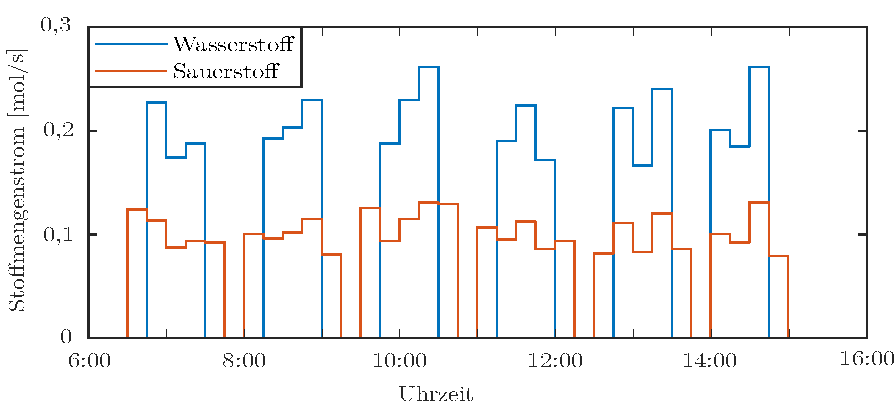
\includegraphics[scale=1]{Figures/Datensatz1molar}
		\caption{An 2018 angelehnter, exemplarischer Verlauf des Wasserstoff und Sauerstoffbedarfs über einen Arbeitstag.}	
\label{fig:Daten1}	
\end{figure}

\begin{figure}[h]
	\centering
		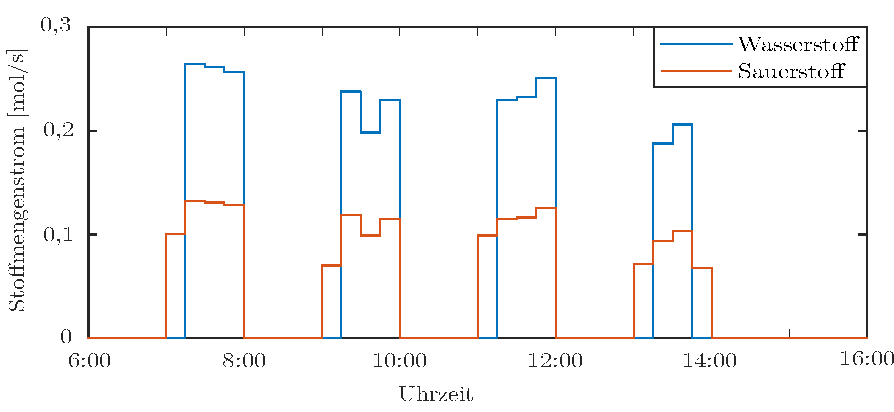
\includegraphics[scale=1]{Figures/Datensatz2molar}
		\caption{An 2019 angelehnter, exemplarischer Verlauf des Wasserstoff und Sauerstoffbedarfs über einen Arbeitstag.}		
\label{fig:Daten2}	
\end{figure}